

\section{问题与应用}

不变性与对称性在源自现实世界的数据中极为常见。因此，21 世纪一些最流行的机器学习应用直接源于几何深度学习并不令人意外，尽管人们有时可能并未充分意识到这一点。
%
我们希望为读者概述几何深度学习中具有影响力的工作以及令人振奋且前景可期的新应用，但这份概述绝非面面俱到。这样做有两个目的：一是展示五类几何域经常出现于哪些具体的科学与工业问题中，二是进一步说明研究几何深度学习原理与架构的必要性。



\paragraph{化学与药物设计} 图上表示学习最具前景的应用之一，是计算化学和\emph{药物开发}。\marginnote{许多药物并非经由设计而得，而是被发现的，且往往出于偶然。多种药物在历史上源自植物界，这一点也反映在它们的名称中。例如，%ephedrine takes its name from the plant genus {\em Ephedra}, atropine from the belladonna plant ({\em Atropa belladonna}), and
通常称为\emph{阿司匹林}的乙酰水杨酸存在于白柳（\emph{Salix alba}）树皮中，而其药用性质自古便为人所知。
} 
%
传统药物是经过设计的小分子，
旨在以化学方式附着（“结合”）到某个靶分子（通常是蛋白质）上，从而激活或阻断某种与疾病相关的化学过程。
%
遗憾的是，药物开发是一个极其漫长且昂贵的过程：
在本文写作之时，
一种新药上市通常需要十年以上，耗资超过十亿美元。
%
原因之一是测试成本；
许多药物会在不同阶段失败——能够进入最后阶段的候选药物不足 5\%（例如见 \cite{gaudelet2020utilising}）。




由于化学上可合成分子的空间极其庞大（估计约为 $10^{60}$），无法通过实验搜索同时具备适当靶标结合亲和力、低毒性、溶解性等性质的候选分子，因而需要采用\emph{虚拟筛选}或\emph{计算机模拟筛选}（即用计算技术识别有前景的分子）。机器学习技术在这项任务中发挥着日益重要的作用。
%
%
\citet{stokes2020deep} 最近给出了几何深度学习用于虚拟药物筛选的一个突出实例：%have definitively demonstrated that this is possible:
他们训练图神经网络预测候选分子能否抑制模式细菌 \emph{Escherichia coli} 的生长，\marginnote{ 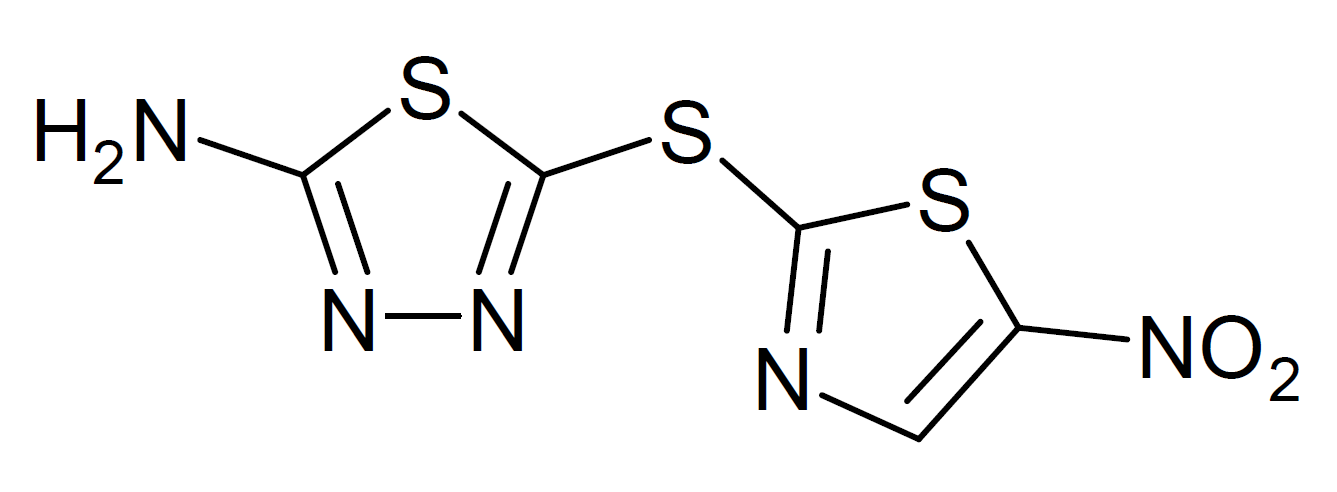
\includegraphics[width=\linewidth]{figures/Halicin_structure.png}\\ Halicin 的分子图。}并由此有效发现，原本适用于治疗糖尿病的分子 \emph{Halicin} 是一种强效抗生素，甚至能够对抗已知具有抗生素耐药性的细菌菌株。这一发现得到了科学媒体和大众媒体的广泛报道。


更广泛地说，把图神经网络应用于建模为图的分子一直是一个非常活跃的领域。近期提出的多种专门架构受到物理学启发，例如纳入了对旋转和平移的等变性（例如见 \cite{thomas2018tensor,anderson2019cormorant,fuchs2020se,satorras2021n}）。此外，\citet{bapst2020unveiling} 成功证明了 GNN 在玻璃动力学预测建模中的效用，其性能超过了此前已有的物理模型。
%
从历史上看，计算化学中的许多工作都是现代图神经网络架构的先驱，并与后者具有许多共同特征。




\paragraph{药物再定位}
%
%\marginnote}---being able to detect novel therapeutics for existing or emerging diseases---commonly by analysing the candidate drug's molecular graph. 
尽管生成全新的候选药物可能是一条可行路径，但开发新疗法还有一种更快、更经济的途径，即\emph{药物再定位}：评估已获批准的药物（单独使用或联合使用）能否用于新的目的。
%
这通常能显著减少药物上市所必需的临床评估。%
在某种抽象层次上，药物对人体生物化学过程的作用，以及药物彼此之间和与其他生物分子的相互作用，都可以建模为图。由此产生了著名网络科学家 Albert-L{\'a}szl{\'o} Barab{\'a}si 提出的“网络医学”概念；该概念主张利用生物网络（如蛋白质--蛋白质相互作用网络和代谢通路）开发新疗法 \citep{barabasi2011network}。


几何深度学习为这类方法提供了现代化视角。一个突出的早期实例是 \cite{zitnik2018modeling} 的工作：他们使用图神经网络预测一种称为\emph{组合疗法}或\emph{多重用药}的药物再定位方案所产生的副作用，并把该问题表述为药物--药物相互作用图中的边预测。
%
在本文写作时仍大范围持续的新型冠状病毒疫情，使人们对以下方向产生了特别浓厚的兴趣：%detecting novel therapeutics; see, e.g.,
尝试应用这类方法对抗 COVID-19 \citep{gysi2020network}。
%
最后需要指出，药物再定位未必局限于合成分子：\cite{veselkov2019hyperfoods} 把类似方法用于食物中所含的类药分子（正如前面提到的，许多植物性食物含有肿瘤治疗所用化合物的生物类似物）。
%
本文的一位作者参与了一项为该研究增添创意的合作：与一位分子料理厨师合作，利用富含这类类药分子的“超级食物”食材设计令人兴奋的菜谱。


\paragraph{蛋白质生物学}
既然已经提到作为药物靶标的蛋白质，我们不妨再花一些篇幅讨论这一主题。
%
蛋白质可以说是最重要的一类生物分子，
%often called the ``molecules of life'', as we are currently not aware of any life-form that is not protein-based. Proteins are encoded in our DNA and 
在人体内承担着无数功能，包括抵御病原体（抗体）、赋予皮肤结构（胶原蛋白）、向细胞输送氧气（血红蛋白）、催化化学反应（酶）以及传递信号（许多激素都是蛋白质）。
%
从化学角度看，蛋白质是一种生物聚合物，即由称为\emph{氨基酸}的小型构件组成的链；它在静电力作用下折叠成复杂的 3D 结构。正是这种结构赋予了蛋白质功能，\marginnote{一个常见比喻可追溯到化学诺贝尔奖得主 Emil Fischer 提出的\emph{Schl{\"u}ssel-Schloss-Prinzip}（“钥匙--锁原理”，1894 年）：两个蛋白质往往只有在几何结构和化学结构互补时才会相互作用。}因此，它对于理解蛋白质如何工作及其功能至关重要。由于蛋白质是药物治疗的常见靶标，%(typical drugs are small molecules designed to bind to their target),
制药行业对这一领域抱有浓厚兴趣。

%\michael{Put AlphaFold here? }

蛋白质生物信息学中的典型问题层次，是从蛋白质\emph{序列}（由 20 种不同氨基酸构成字母表上的 1D 字符串），到 3D \emph{结构}（称为“蛋白质折叠”的问题），再到\emph{功能}（“蛋白质功能预测”）。
%
近期方法（例如 \cite{senior2020improved} 提出的 DeepMind AlphaFold）使用\emph{接触图}表示蛋白质结构。\cite{gligorijevic2020structure} 表明，在这类图上应用图神经网络，能够取得优于纯序列方法的功能预测结果。


\cite{gainza2020deciphering} 开发了名为 MaSIF 的几何深度学习流水线，\marginnote{ 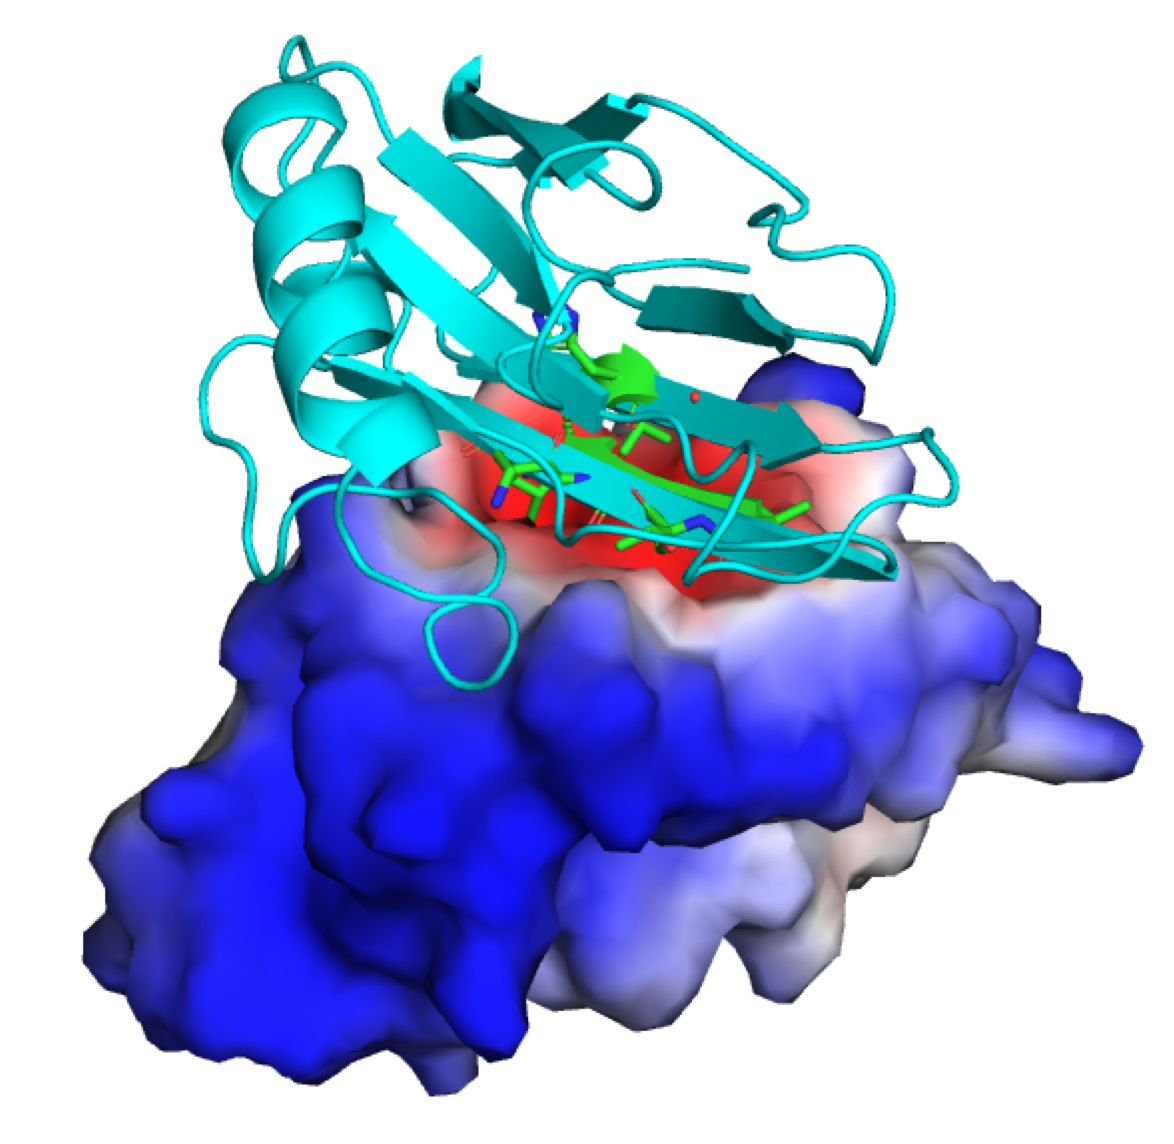
\includegraphics[width=\linewidth]{figures/masif.png}\\ 肿瘤靶标 PD-L1 的蛋白质表面（热图表示预测的结合位点）以及设计得到的结合体（以带状图显示）。}根据蛋白质的 3D 结构预测蛋白质间相互作用。MaSIF 把蛋白质建模为离散成网格曲面的分子表面，并指出这种表示在处理相互作用时具有优势，因为它能够抽象掉内部折叠结构。该架构基于网格曲面卷积神经网络，对小型局部测地线斑块中预先计算的化学与几何特征进行运算。%
该网络使用 Protein Data Bank 中数千个蛋白质共晶 3D 结构进行训练，以处理界面预测、配体分类和对接等多项任务；它还能够\emph{从头}设计理论上可作为抗癌生物免疫治疗药物的蛋白质。这类蛋白质旨在抑制程序性细胞死亡蛋白复合物各部分（PD-1/PD-L1）之间的蛋白质--蛋白质相互作用（PPI），使免疫系统获得攻击肿瘤细胞的能力。%showing state-of-the-art performance.

%A key difference of MaSIF compared to other methods is that it does not rely on the evolutionary history of proteins. This is of crucial importance in de novo protein design, where one tries to create “from scratch” new proteins that have never existed before.



\paragraph{推荐系统与社交网络} 图表示学习最早得到普及的大规模应用出现在\emph{社交网络}\marginnote{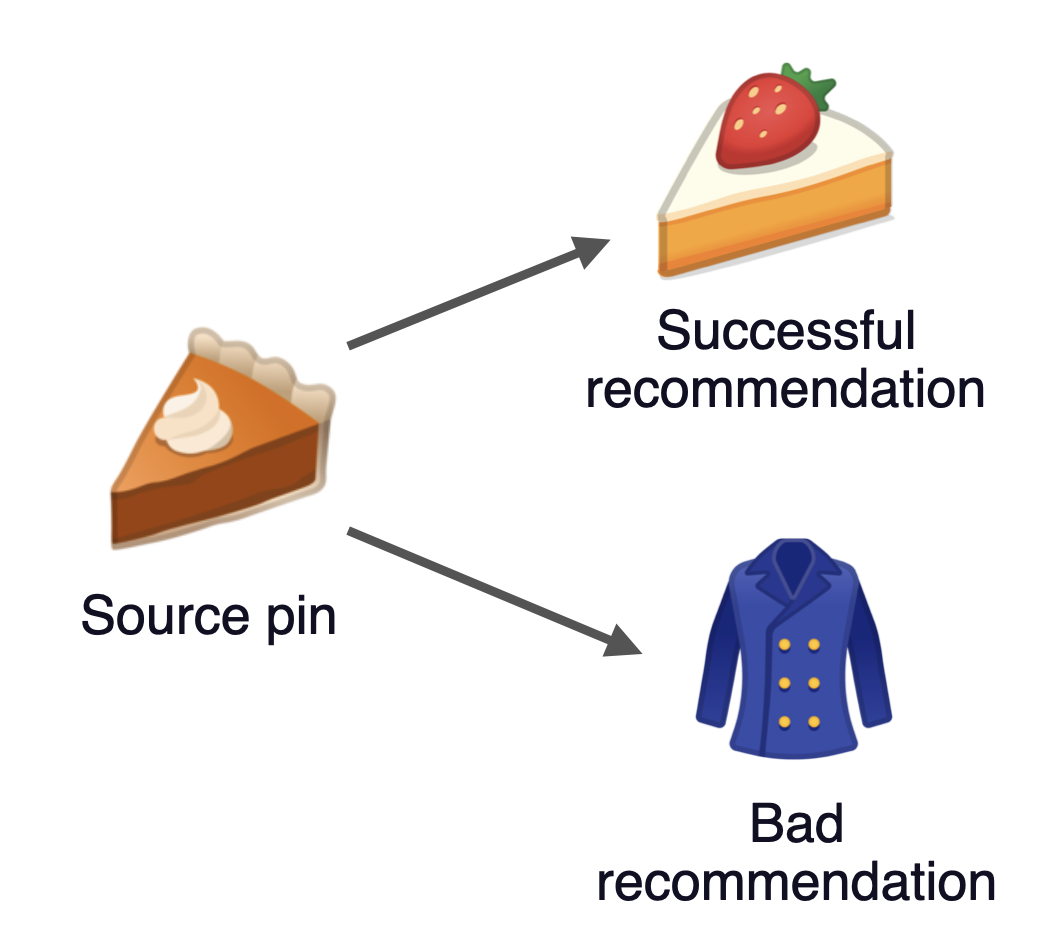
\includegraphics[width=\linewidth]{figures/Recommender.png}}中，主要应用场景是\emph{推荐系统}。推荐器的任务是决定向用户提供哪些内容，这一决定可能取决于用户此前在服务中的交互历史。该任务通常通过\emph{链接预测}目标实现：对各种节点（内容项）的嵌入进行监督，使被认为\emph{相关}的节点（例如经常被共同浏览的内容）彼此接近。于是，两个嵌入的\emph{接近程度}（例如它们的内积）可以解释为二者在内容图中由一条边连接的概率；因此，对于用户查询的任意内容，一种做法是在嵌入空间中提供其 $k$ 个最近邻。

这一方法的先驱之一是美国图片分享与社交媒体公司 Pinterest：除了率先成功地在生产环境中部署 GNN 之外，其 PinSage 方法\marginnote{Pinterest 还提出了后续工作 PinnerSage \citep{pal2020pinnersage}，它把用户特定的上下文信息有效整合进推荐器。}还成功使图表示学习能够\emph{扩展}到拥有数百万节点和数十亿条边的图 \citep{ying2018graph}。相关应用很快相继出现，尤其集中在商品推荐领域。目前部署于生产环境的常见 GNN 推荐器包括 Alibaba 的 Aligraph \citep{zhu2019aligraph} 和 Amazon 的 P-Companion \citep{hao2020p}。图深度学习正以这种方式每天影响着数以百万计的人。


在社交网络内容分析的背景下，另一个值得注意的项目是 Fabula AI；它是最早被收购的 GNN 初创公司之一（2019 年由 Twitter 收购）。这家初创公司由本文的一位作者及其团队创立，开发了检测社交网络错误信息的新技术 \citep{monti2019fake}。Fabula 的方案用分享某条新闻的用户网络来建模该新闻的传播过程：如果一个用户转发了另一个用户的信息，或者两人在社交网络上相互关注，就在二者之间建立连接。随后将该图输入图神经网络，由网络把整个图分类为“真实”或“虚假”内容；标签依据事实核查机构之间的共识给出。该方法不仅展现出强大且很快趋于稳定的预测能力（通常在新闻开始传播后的数小时内），对各个用户节点嵌入的分析还揭示出倾向于分享错误信息的用户形成了明显聚类，这正体现了众所周知的\emph{“回音室”}效应。

\paragraph{交通预测} 交通运输网络是几何深度学习技术已经对全球数十亿用户产生实际影响的另一个领域。\marginnote{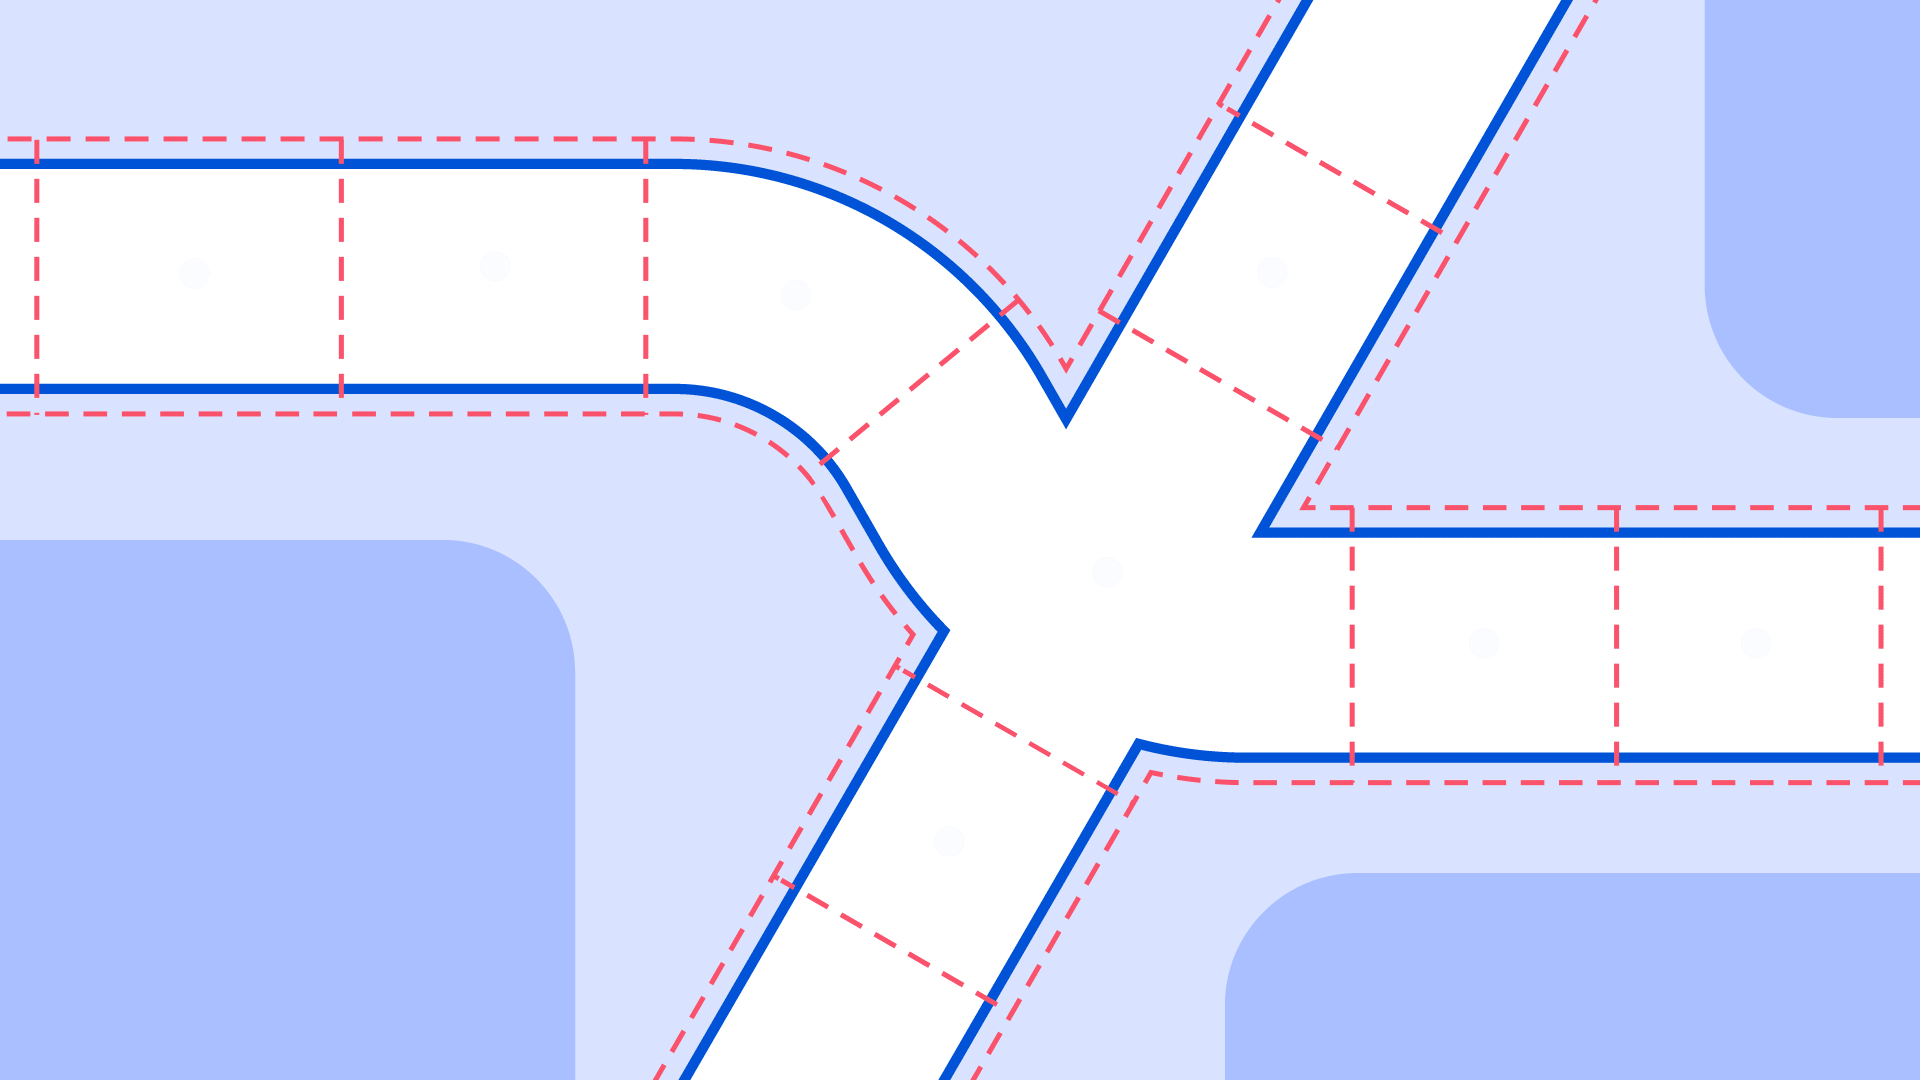
\includegraphics[width=\linewidth]{figures/superseg-1.png}\\ 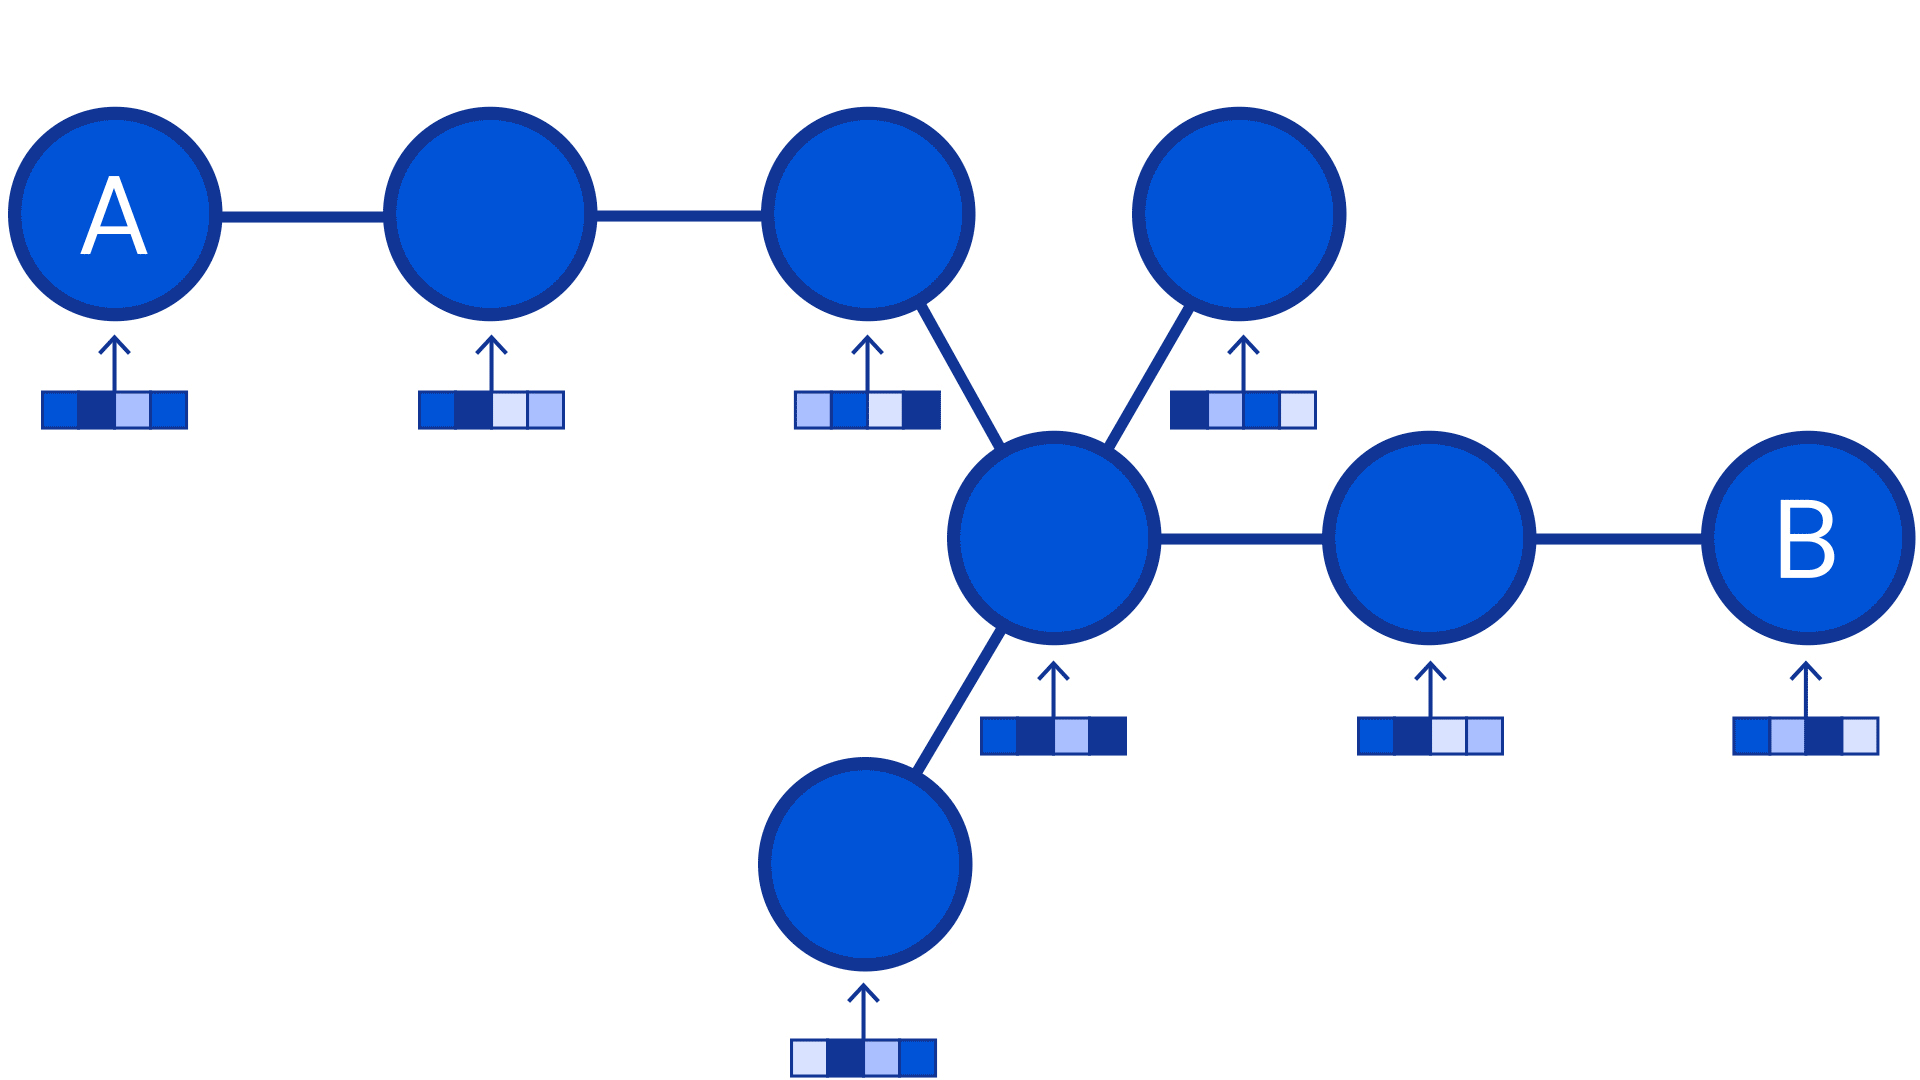
\includegraphics[width=\linewidth]{figures/superseg-3.png}\\ 道路网络（上）及其对应的图表示（下）。}例如，在道路网络上，可以把交叉路口视为节点，把连接它们的路段视为边；随后可用道路长度、路段当前或历史行驶速度等信息为这些边构造特征。

这一领域的标准预测问题之一是预测\emph{预计到达时间}（ETA）：对于给定的候选路线，提供走完该路线所需的预期行程时间。这个问题至关重要，不仅涉及面向用户的交通推荐应用，也关系到在自身运营中使用这类预测的企业（如外卖或网约车服务）。

图神经网络在这一领域同样展现出巨大潜力：例如，可直接预测道路网络相关子图的 ETA（实质上是一项\emph{图回归}任务）。\marginnote{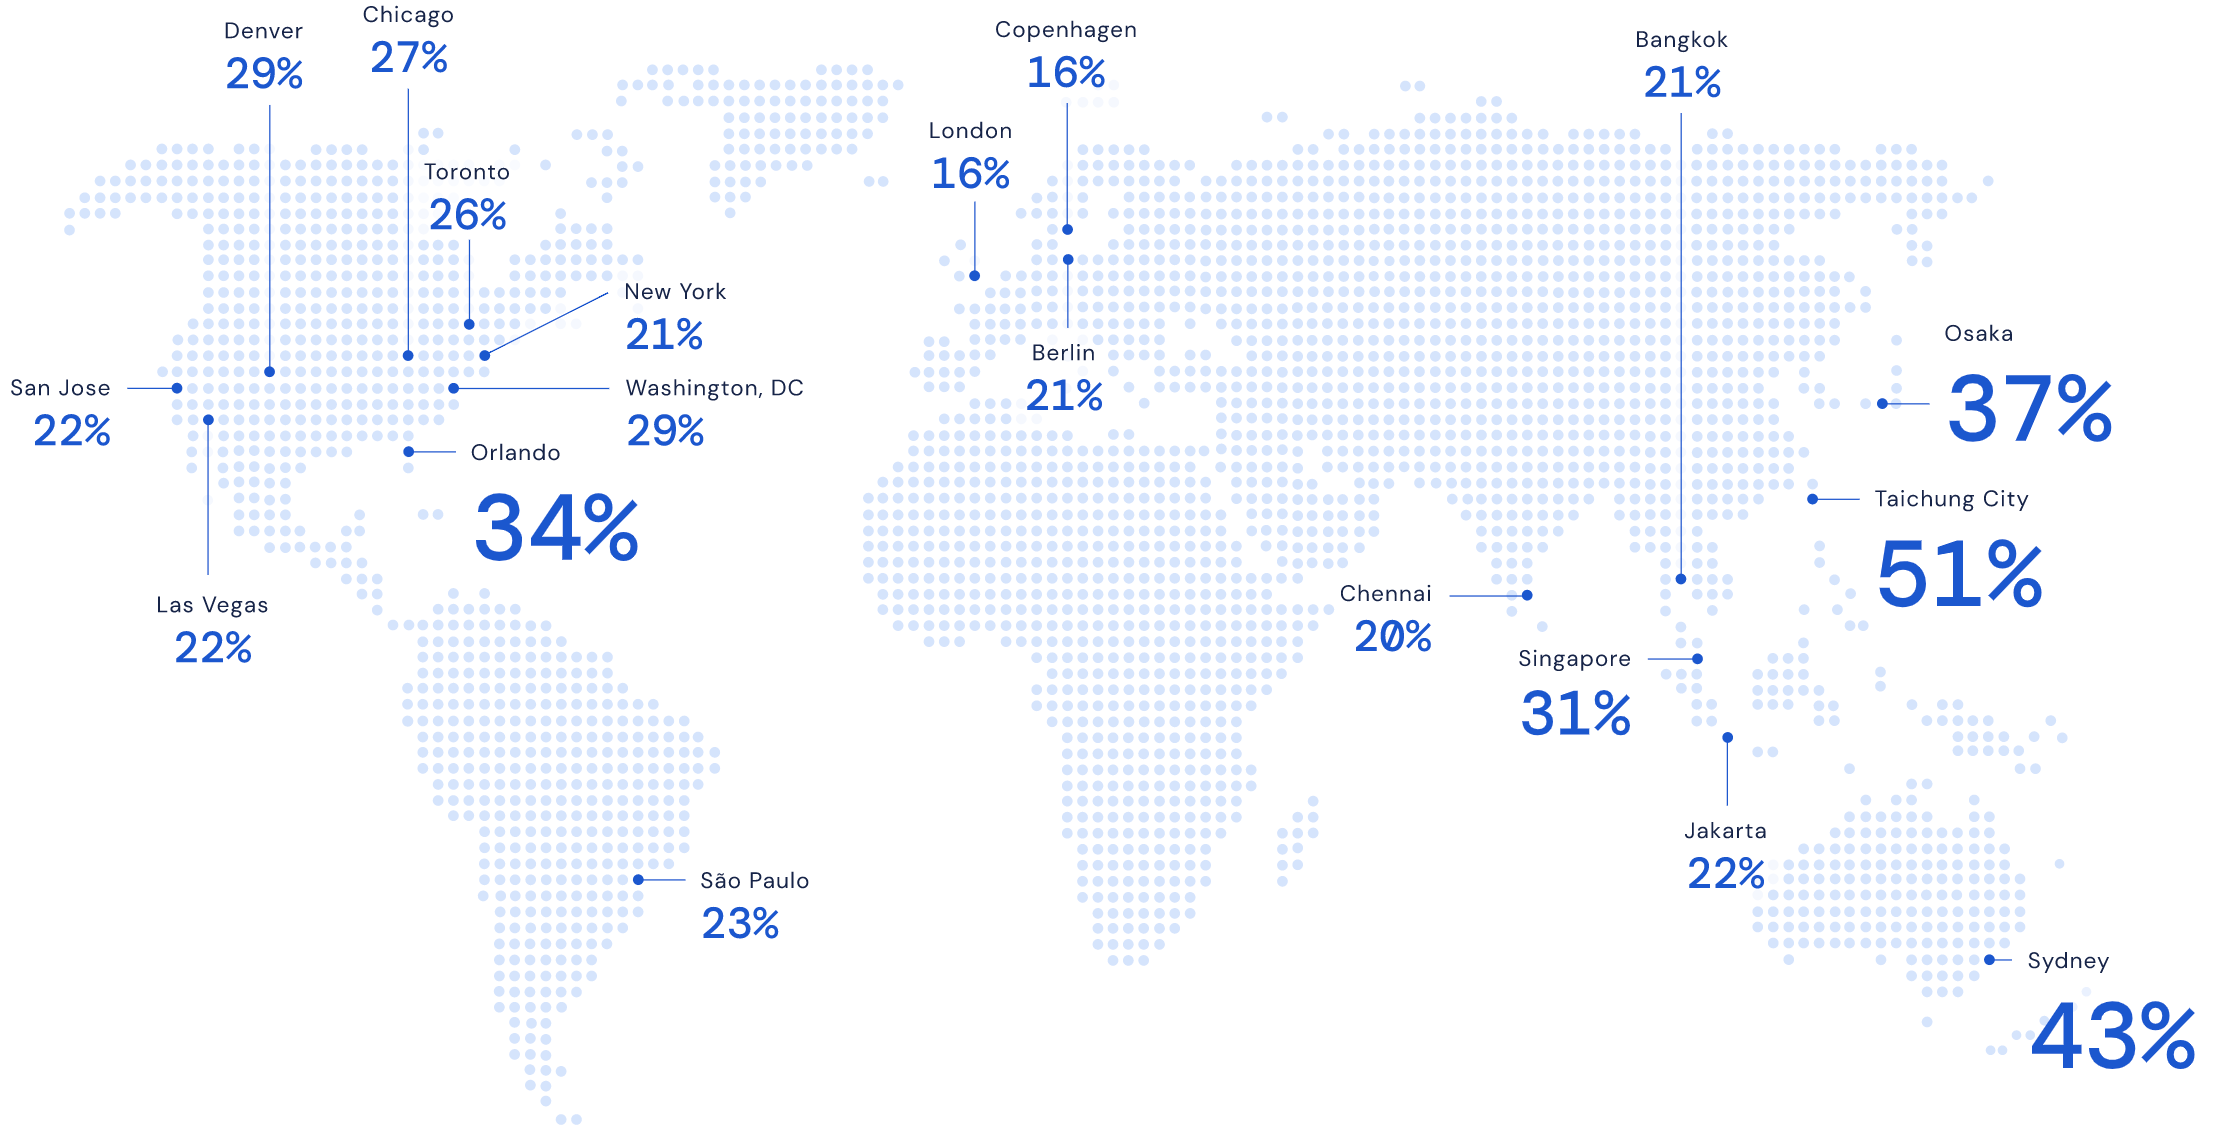
\includegraphics[width=\linewidth]{figures/maps-improvements.png}\\ Google Maps 中使用 GNN 响应查询的若干大都市区域，并标出了预测质量的相对提升（Sydney 等城市达到 40+\%）。}DeepMind 成功采用了这种方法，得到一个基于 GNN 的 ETA 预测器；该预测器现已部署在 Google Maps 的生产环境中，为全球多个主要都市区提供 ETA 查询服务 \citep{derrowpinion2021traffic}。Baidu Maps 团队也观察到类似收益；其行程时间预测目前由 ConSTGAT 模型提供，而该模型本身基于图注意力网络模型的一种时空变体 \citep{fang2020constgat}。

\paragraph{物体识别} 计算机视觉中机器学习技术的一项主要基准，是能否对给定图像中的中心物体进行\emph{分类}。\marginnote{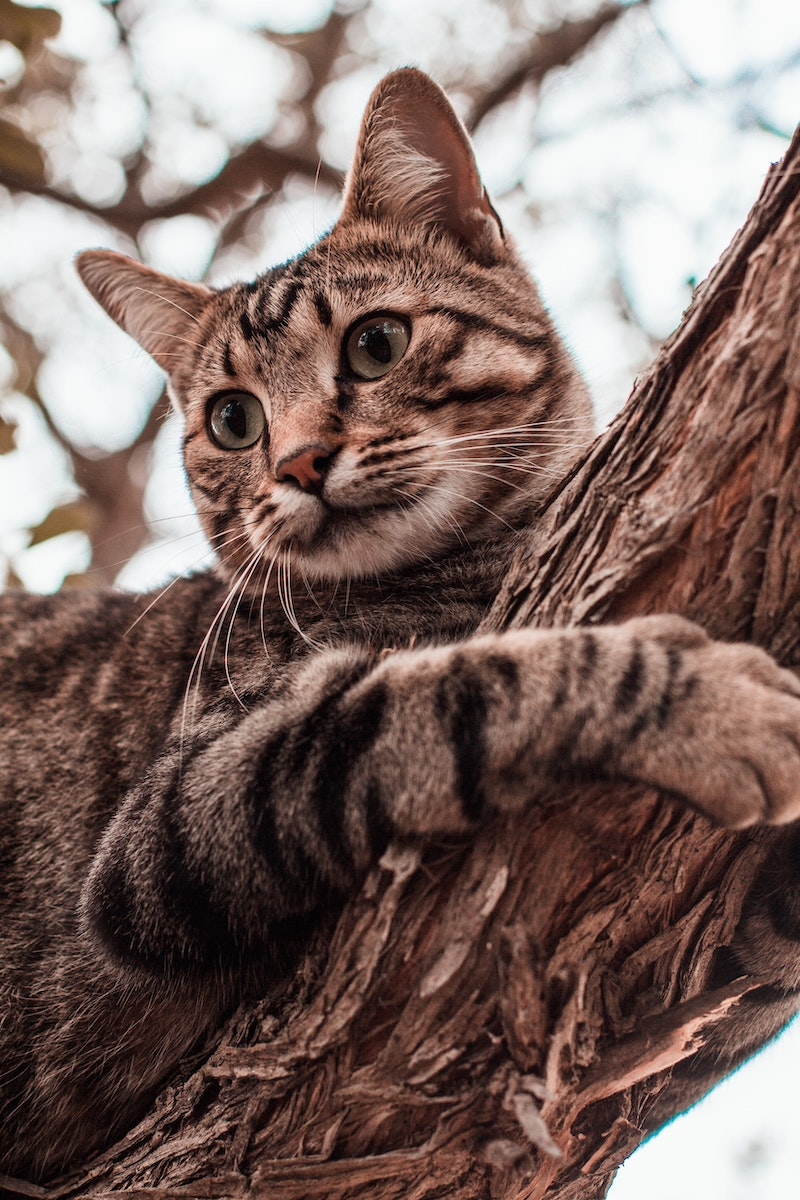
\includegraphics[width=\linewidth]{figures/tabby_cat.jpg}\\ 一幅输入图像示例；ImageNet 中可以找到类似图像，它表示\emph{“虎斑猫”}类别。}ImageNet 大规模视觉识别挑战赛 \citep[ILSVRC]{russakovsky2015imagenet} 是一项年度物体分类竞赛，推动了几何深度学习早期发展的很大一部分。ImageNet 要求模型把从 Web 抓取的真实图像分到 1000 个类别之一：这些类别既多样（涵盖有生命和无生命物体），又具体（许多类别着重区分不同的猫和犬品种）。因此，在 ImageNet 上表现良好往往意味着模型能够从一般照片中稳健地提取特征，这为从预训练 ImageNet 模型出发的各种\emph{迁移学习}设置奠定了基础。

卷积神经网络在 ImageNet 上的成功——尤其是 \citet{krizhevsky2012imagenet} 的 AlexNet 模型在 ILSVRC 2012 中以巨大优势夺冠——在很大程度上引领了整个深度学习在学术界和工业界的应用。此后，CNN 一直位居 ILSVRC 前列，并催生了许多流行架构，如 VGG-16 \citep{simonyan2014very}、\marginnote{有趣的是，VGG-16 架构有十六个卷积层，作者称其为“非常深”。随后的发展很快把这类模型扩展到数百层乃至数千层。}[5\baselineskip]Inception \citep{szegedy2015going} 和 ResNets \citep{he2016deep}；这些架构已在该任务上成功超越人类水平。这些架构采用的设计决策与正则化技术（如修正线性激活 \citep{nair2010rectified}、dropout \citep{srivastava2014dropout}、跳跃连接 \citep{he2016deep} 和批归一化 \citep{ioffe2015batch}）构成了当今许多有效 CNN 模型的基础。

在物体分类发展的同时，物体\emph{检测}也取得了显著进展；它要求分离出图像中所有感兴趣的物体，并为它们标注特定类别。该任务关系到从图像描述到自动驾驶汽车的多种下游问题。由于预测结果需要\emph{局部化}，它要求采用更细粒度的方法；因此，平移等变模型往往在这一领域体现出价值。一个有影响力的实例是 R-CNN 模型家族 \citep{girshick2014rich,girshick2015fast,ren2015faster,he2017mask}。在相关的\emph{语义分割}领域，\citet{badrinarayanan2017segnet} 的 SegNet 模型也颇具影响力，其编码器--解码器架构以 VGG-16 为骨干。

\paragraph{游戏博弈} 当观测状态能够表示在网格域上时，卷积神经网络也作为平移不变特征提取器，在\emph{强化学习}（RL）环境中发挥重要作用；例如，从像素学习玩电子游戏便属于这种情况。%\marginnote{\includegraphics[width=0.9\linewidth]{figures/mspacman.png} The \emph{Atari 2600} is an example of a video gaming system that has been heavily repurposed as an RL environment (primarily by the efforts of \citet{bellemare2013arcade}. Shown above is an image of \emph{Ms. Pacman}, one of the games supported therein.}.
%
在这种情况下，CNN 负责把输入约化为扁平向量表示，随后用该表示导出驱动 RL 智能体行为的\emph{策略}或\emph{价值函数}。尽管强化学习的具体细节并非本节重点，但需要指出，过去十年中一些最具影响力的深度学习成果来自以 CNN 为支撑的强化学习。

这里尤其值得提及的一个实例是 DeepMind 的 \emph{AlphaGo} \citep{silver2016mastering}。它把 CNN 应用于表示当前棋子位置的 $19\times 19$ 网格，从而编码围棋对局的当前状态。随后，通过结合学习既往专家棋步、Monte Carlo 树搜索和自我对弈，它成功达到足以在五局挑战赛中击败 Lee Sedol 的围棋水平；后者是有史以来最强的围棋棋手之一，这场比赛也得到了全球广泛报道。

这已经是更广泛人工智能领域的一个重要里程碑——围棋的状态空间远比国际象棋等游戏复杂。\marginnote{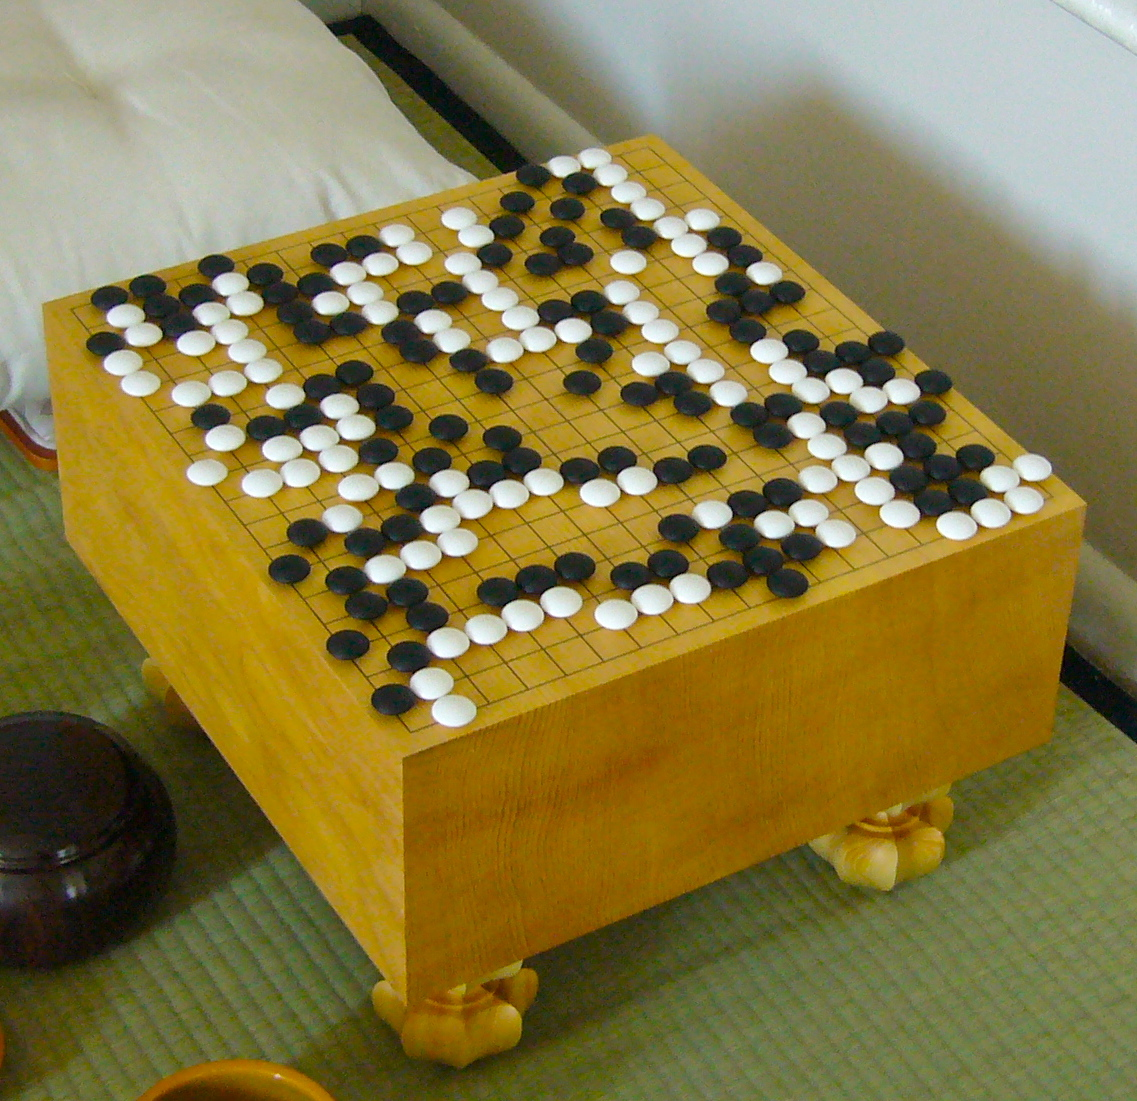
\includegraphics[width=\linewidth]{figures/Go_board.jpeg} 围棋在 $19\times 19$ 棋盘上进行，两名棋手在空位放置黑白\emph{棋子}。合法状态数估计为 $\approx2\times 10^{170}$ \citep{tromp2006combinatorics}，远远超过宇宙中的原子数。}但 AlphaGo 的发展并未就此止步。作者逐步从架构中移除越来越多围棋特有的偏置：\emph{AlphaGo Zero} 移除了人类偏置，仅通过自我对弈进行优化 \citep{silver2017mastering}；\emph{AlphaZero} 把该算法扩展到国际象棋和将棋等相关双人游戏；最后，\emph{MuZero} \citep{schrittwieser2020mastering} 纳入了一个能够即时\emph{学习}游戏规则的模型，从而在没有任何先验规则知识的情况下，在 Atari 2600 游戏以及围棋、国际象棋和将棋上取得强劲性能。在所有这些发展过程中，CNN 始终是这些模型表示输入的骨干。

多年来，人们为 Atari 2600 平台提出了多个高性能 RL 智能体 \citep{mnih2015human,mnih2016asynchronous,schulman2017proximal}，但它们长期无法在该平台提供的\emph{全部} 57 款游戏上达到人类水平。Agent57 \citep{badia2020agent57} 最终突破了这一障碍：它使用从强探索性到纯利用性的参数化策略族，并在不同训练阶段以不同方式确定这些策略的优先级。它的大部分计算同样由作用于电子游戏帧缓冲区的 CNN 完成。

\paragraph{文本与语音合成} 除了自然映射到\emph{二维}网格的图像之外，（几何）深度学习的一些重大成功发生在一维网格上。\emph{文本}和\emph{语音}便是自然的例子，它们把几何深度学习蓝图带入自然语言处理和数字信号处理等不同领域。

这一领域中应用最广、报道最多的一些工作聚焦于\emph{合成}：无条件地，或以特定\emph{提示}为条件，生成语音或文本。这种设置可以支持大量实用任务，如\emph{文本转语音}（TTS）、预测式文本补全和机器翻译。过去十年中，人们提出了多种文本与语音生成神经架构；早期方案大多基于\emph{循环}神经网络，例如前述 seq2seq 模型 \citep{sutskever2014sequence} 或循环注意力 \citep{bahdanau2014neural}。然而，近年来它们逐渐被卷积神经网络和基于 Transformer 的架构取代。

这一设置中，简单 1D 卷积的一项特有限制是其\emph{感受野}线性增长，因而需要许多层才能覆盖此前已经生成的序列。相比之下，\emph{空洞}卷积\marginnote{空洞卷积也称为 \emph{\`{a} trous} 卷积（该法语词组字面意为“带孔的”）。}能以相同数量的参数提供\emph{指数增长}的感受野。凭借这一点，它成为非常有力的替代方案，最终在机器翻译上达到可与 RNN 竞争的水平 \citep{kalchbrenner2016neural}；同时，由于能够在所有输入位置并行计算，它还大幅降低了计算复杂度。\marginnote{这类技术在蛋白质--蛋白质相互作用等不同问题上也超过了 RNN \citep{deac2019attentive}。}空洞卷积最知名的应用是 \cite{oord2016wavenet} 提出的 \emph{WaveNet} 模型。WaveNet 证明，利用空洞可以在\emph{原始波形}层面（通常每秒 16,000 个或更多采样点）合成语音，所生成的语音样本比此前最好的文本转语音（TTS）系统明显更“像人”。\marginnote{除此之外，WaveNet 模型还被证明能够生成钢琴曲。}随后，研究进一步表明，可以把 WaveNet 的计算蒸馏到简单得多的 \emph{WaveRNN} 模型 \citep{kalchbrenner2018efficient} 中；该模型使这项技术能够有效地实现工业规模部署。这不仅使其能够用于 Google Assistant 等服务的大规模语音生成，也使 Google Duo 等使用端到端加密的应用能够在设备端高效计算。

Transformer \citep{vaswani2017attention} 成功突破了循环架构与卷积架构的限制，表明仅凭\emph{自注意力}即可在机器翻译中取得最先进性能。随后，Transformer 给自然语言处理带来了革命性变化。借助 BERT \citep{devlin2018bert} 等模型提供的预训练嵌入，Transformer 计算得以用于大量自然语言处理下游应用；例如，Google 使用 BERT 嵌入为其搜索引擎提供支持。

过去几年中，Transformer 得到最广泛报道的应用或许是文本生成；这一方向主要由 OpenAI 的\emph{生成式预训练 Transformer}（GPT，\cite{radford2018improving,radford2019language,brown2020language}）模型家族推动。特别是，GPT-3 \citep{brown2020language} 成功把语言模型学习扩展到 1750 亿个可学习参数，并使用 Web 规模的抓取文本语料进行下一词预测训练。这使它不仅成为能在多种语言任务上发挥强大作用的少样本学习器，还成为能够生成连贯且近似人类表达的文本生成器。这种能力既带来了大量下游应用，也引发了广泛的媒体报道。

\paragraph{医疗健康}
%
医疗领域的应用是几何深度学习另一个前景可期的方向。这些方法正以多种方式得到使用。
%
首先，CNN 等较传统的架构已被应用于网格结构数据，例如用于
预测重症监护病房的住院时长
\citep{rocheteau2020temporal}, 
或根据视网膜扫描诊断威胁视力的疾病 \citep{de2018clinically}。
%
\cite{winkels2019pulmonary} 表明，与常规 CNN 相比，使用 3D 旋转--平移群卷积网络能够提高
肺结节检测的准确率。


其次，把器官建模为几何曲面后，网格曲面卷积神经网络已被证明能够处理多种任务，包括根据遗传学相关信息重建面部结构 \citep{mahdi20203d}、
大脑皮层分区 \citep{cucurull2018convolutional}，以及
根据皮层表面结构回归人口统计学属性 \citep{besson2020geometric}。
%
%The latter problems consists of []
%Third, 
%
后一组例子体现了神经科学中日益明显的一种趋势：把大脑视为具有复杂褶皱的曲面，\marginnote{在解剖学文献中，大脑皮层的这类结构称为\emph{脑沟}和\emph{脑回}。}由此产生高度非 Euclidean 的结构。
%since the data in this field are often represented on surface models of the brain. 
%as many cortical properties only make sense considering their specific location with respect to the various sulci and gyri [8]. These surface models are essentially sheet-like meshes that are intricately folded in three-dimensional space, maintaining the geometrical structure of the brain


与此同时，
神经科学家经常尝试构建并分析大脑的\emph{功能网络}，表示执行某种认知功能时共同激活的各个脑区；这些网络通常用功能磁共振成像（fMRI）构建，该技术实时显示大脑哪些区域消耗了更多血液。\marginnote{通常使用血氧水平依赖（BOLD）对比成像。}
%
这些功能网络既可以揭示患者的人口统计学特征（例如区分男性与女性，\cite{arslan2018graph}），也可以用于神经病理诊断；后者是我们要在此强调的几何深度学习在医学中的第三类应用。在这一背景下，\cite{ktena2017distance} 率先使用图神经网络预测孤独症谱系障碍等神经系统疾病。
%
大脑的几何结构与功能结构似乎密切相关，近期 \cite{itani2021combining} 指出，在神经系统疾病分析中联合利用二者是有益的。
% can reveal important information about the complexity of the neuropathology


第四，\emph{患者网络}在基于 ML 的医学诊断中正变得更加重要。这类方法的基本依据是，患者在人口统计学、基因型和表型上的相似性信息可能有助于改善疾病预测。
%
 \cite{parisot2018disease}
 把图神经网络应用于由人口统计学特征构建的患者网络，以诊断神经系统疾病，并表明使用图能够改善预测结果。
 %
\cite{cosmo2020latent} 展示了潜在图学习（即由网络\emph{学习}未知的患者图）在这一设置中的益处。后一项工作使用了 UK Biobank 的数据；这是一个包含脑成像在内的大规模医学数据集合 \citep{miller2016multimodal}。




医院患者的大量数据可以在\emph{电子健康记录}（EHR）中找到。\marginnote{公开可用的匿名重症监护 EHR 数据集包括 MIMIC-III \citep{johnson2016mimic} 和 eICU \citep{pollard2018eicu}。}EHR 分析不仅能够全面呈现患者的病情发展，还能把相似患者\emph{关联}起来。这与诊断中常用的\emph{模式识别法}一致：临床医生凭借\emph{经验}识别临床特征模式；当医生的经验使其能够迅速诊断病情时，这可能就是所采用的主要方法。沿着这一思路，多项工作尝试基于 EHR 数据构建患者图，其依据可以是医生记录的嵌入 \citep{malone2018learning}、入院时诊断的相似性 \citep{rocheteau2021predicting}，甚至可以假定一个全连接图 \citep{zhu2019graph}。在所有这些情形中，使用图表示学习处理 EHR 都展现出了有前景的结果。



\paragraph{粒子物理学与天体物理学}
高能物理学家或许是自然科学领域最早接纳图神经网络这一崭新工具的专业群体之一。
%
在近期的一篇综述中，\cite{shlomi2020graph} 指出，\marginnote{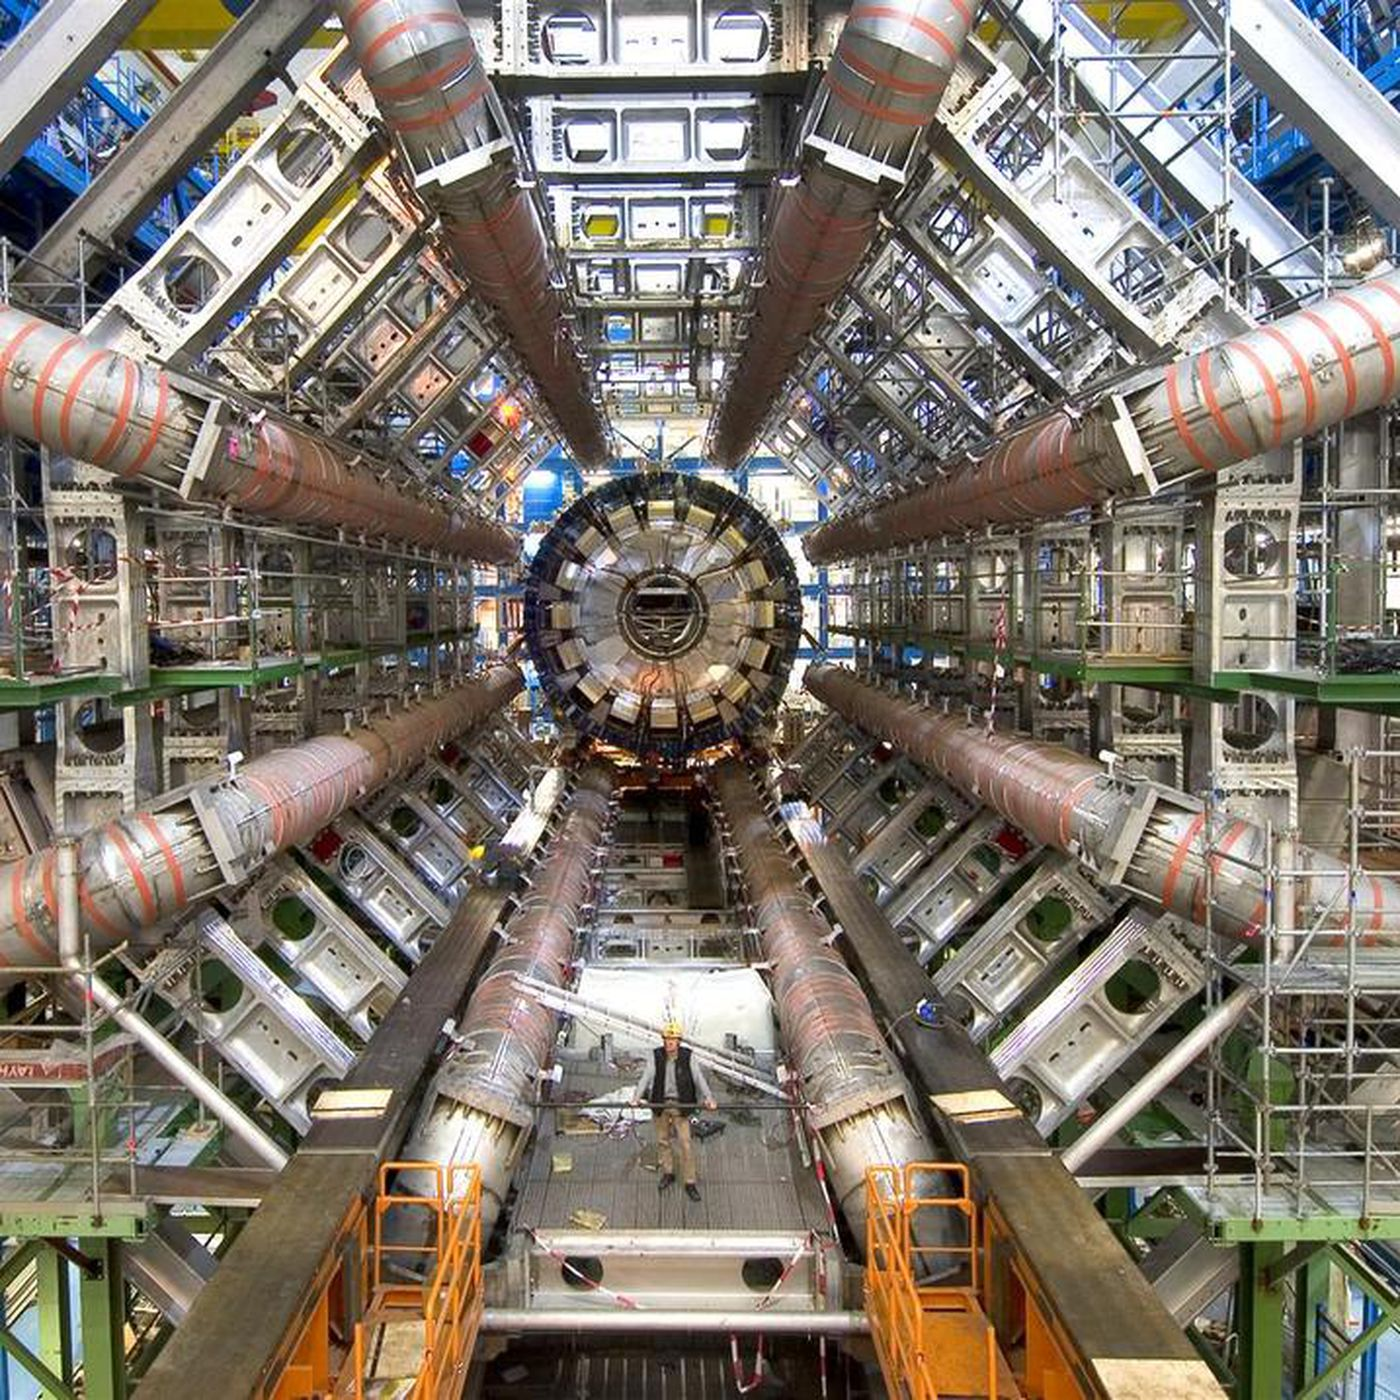
\includegraphics[width=\linewidth]{figures/lhc.jpeg}
Large Hadron Collider 探测器的一部分。
}机器学习在粒子物理实验中历来得到广泛使用：或者学习复杂的逆函数，以便从探测器测得的信息推断底层物理过程；或者执行分类与回归任务。对于后一类任务，为了能够使用 CNN 等标准深度学习架构，往往必须强行把数据转化为网格等不自然的表示。然而，物理学中的许多问题涉及无序集合形式的数据，其中包含丰富的关系与相互作用，因此可以自然地表示为图。


高能物理学的一项重要应用是重建并分类\emph{粒子喷注}——它们是稳定粒子形成的喷流，%that are stemming
源于某一初始事件所产生粒子的多次连续相互作用与衰变。
% (for example, a collision of ).
%
在 CERN 建造的最大、最著名的粒子加速器 Large Hadron Collider 中，这类喷注源自以接近光速运动的质子之间的碰撞。
%ccelerated to a speed close to that of light, they collide with other protons. 
这些碰撞会产生有质量粒子，例如长期以来人们一直在寻找的 Higgs 玻色子或顶夸克。
%
%object. 
%
识别并分类碰撞事件至关重要，因为这可能为新粒子的存在提供实验证据。


近期，人们为粒子喷注分类任务提出了多种几何深度学习方法；\marginnote{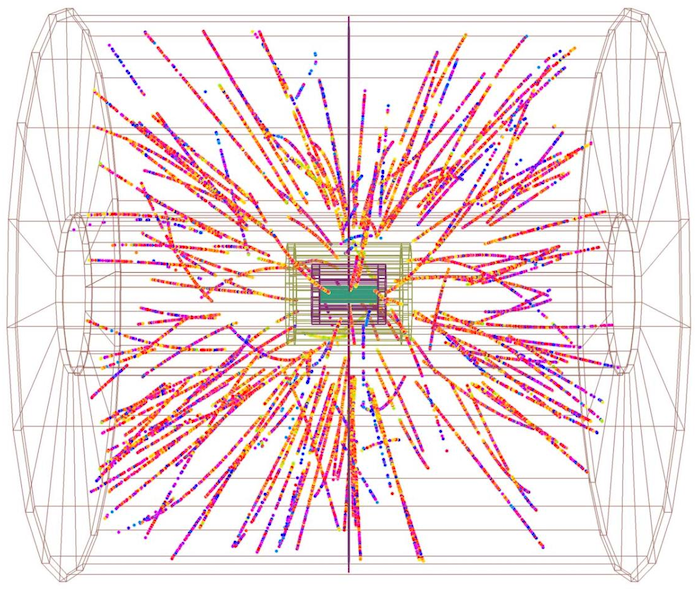
\includegraphics[width=\linewidth]{figures/particlejet.png}
粒子喷注示例。
}例如，\cite{komiske2019energy} 和 \cite{qu1902particlenet} 分别提出了基于 DeepSet 和 Dynamic Graph CNN 架构的方法。
%
%Recently GNNs have been extended by adding inductive biases
近来，人们还对开发源于物理学考虑的专门架构产生了兴趣：这类架构可以纳入与 Hamilton 或 Lagrange 力学一致的归纳偏置（例如见 \cite{sanchez2019hamiltonian,cranmer2020lagrangian}），对 Lorentz 群（物理学中时空的一项基本对称性）保持等变 \citep{bogatskiy2020lorentz}，甚至纳入符号推理 \citep{cranmer2019learning}，并能够从数据中学习物理定律。这类方法更具可解释性（因而被领域专家视为更“可信”），也具有更好的泛化能力。



除了粒子加速器之外，
天体物理学家如今还把粒子探测器用于\emph{多信使天文学}——这是一种协调观测来自同一信号源的电磁辐射、引力波和中微子等不同信号的新方式。
%
中微子天文学尤其引人关注，因为中微子极少与物质发生相互作用，因而能够几乎不受影响地传播极远距离。\marginnote{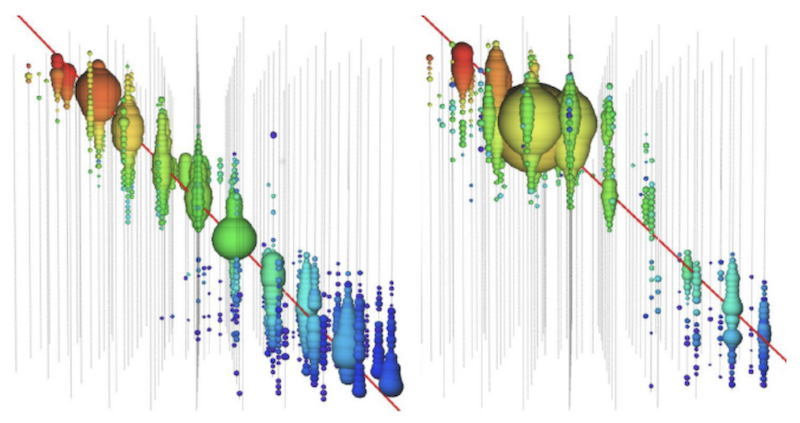
\includegraphics[width=\linewidth]{figures/icecube.png} IceCube 探测器中背景事件（左：muon 束）
与天体物理中微子（右：高能单 muon）形成的特征性光沉积分布。\cite{choma2018graph}
}探测中微子可以观测光学望远镜无法观测的对象，但需要规模极其庞大的探测器——IceCube 中微子观测站使用南极点一立方千米的南极冰架作为探测器。
%
探测高能中微子可能有助于揭示宇宙中一些最神秘的对象，例如耀变体和黑洞。
%
\cite{choma2018graph} 使用几何神经网络建模 IceCube 中微子探测器的不规则几何结构，在探测来自天体物理源的中微子并将其与背景事件分离方面展现出显著更好的性能。


尽管中微子天文学在宇宙研究中前景广阔，传统光学望远镜和射电望远镜仍然是天文学家的主力工具。
%
即使使用这些传统仪器，几何深度学习仍能为数据分析提供新方法。例如，\cite{scaife2021fanaroff} 使用旋转等变 CNN 对射电星系进行分类，\cite{mcewen2021scattering} 则使用
球面 CNN 分析宇宙微波背景辐射；后者是 Big Bang 的遗迹，可能有助于揭示早期宇宙的形成。正如前面提到的，这类信号自然地表示在球面上，而等变神经网络是研究它们的适当工具。


%\michael{TACO: anything on the sphere? There is a work of Defferard, but I don't like it because they use GNNs on the meshed sphere, which is non comme il faut}

%[47], which can improve performance and generalization on various physical
%prediction problems. Other recent work [7] has shown symbolic physical laws can be
%extracted from the learned functions within a GN.


%For additional details on various applications of Geometric Deep Learning in particle physics, we refer the reader to a recent review by \cite{shlomi2020graph}. 



\paragraph{虚拟现实与增强现实}
另一个推动大量几何深度学习方法发展的应用领域是计算机视觉与图形学，尤其是面向虚拟现实和增强现实的 3D 人体模型处理。
%
用于制作 Avatar 等电影特效的动作捕捉技术通常分两个阶段运行：首先，把捕捉演员身体或面部动作的 3D 扫描仪输入与某个规范形状建立对应关系；该形状通常建模为离散流形或网格曲面（这一问题常称为“分析”）。其次，生成一个新形状来复现输入的动作（“合成”）。
%
计算机图形学与视觉中关于几何深度学习的早期工作 \citep{masci2015geodesic,boscaini2016learning,monti2017geometric} 开发了网格曲面卷积神经网络，用于解决分析问题，更具体地说，是可形变形状对应问题。


\cite{litany2018deformable} 和 \cite{ranjan2018generating} 分别独立提出了最早用于 3D 形状合成的几何自编码器架构。在这些架构中，假定身体、面部或手部的规范网格曲面已知，而合成任务则是回归节点的 3D 坐标（用微分几何术语说，即曲面的嵌入）。%,bouritsas2019neural}.
%
\cite{kulon2020weakly} 展示了一条用于 3D 手部姿态估计的混合流水线，它采用基于图像 CNN 的编码器和几何解码器。\marginnote{ 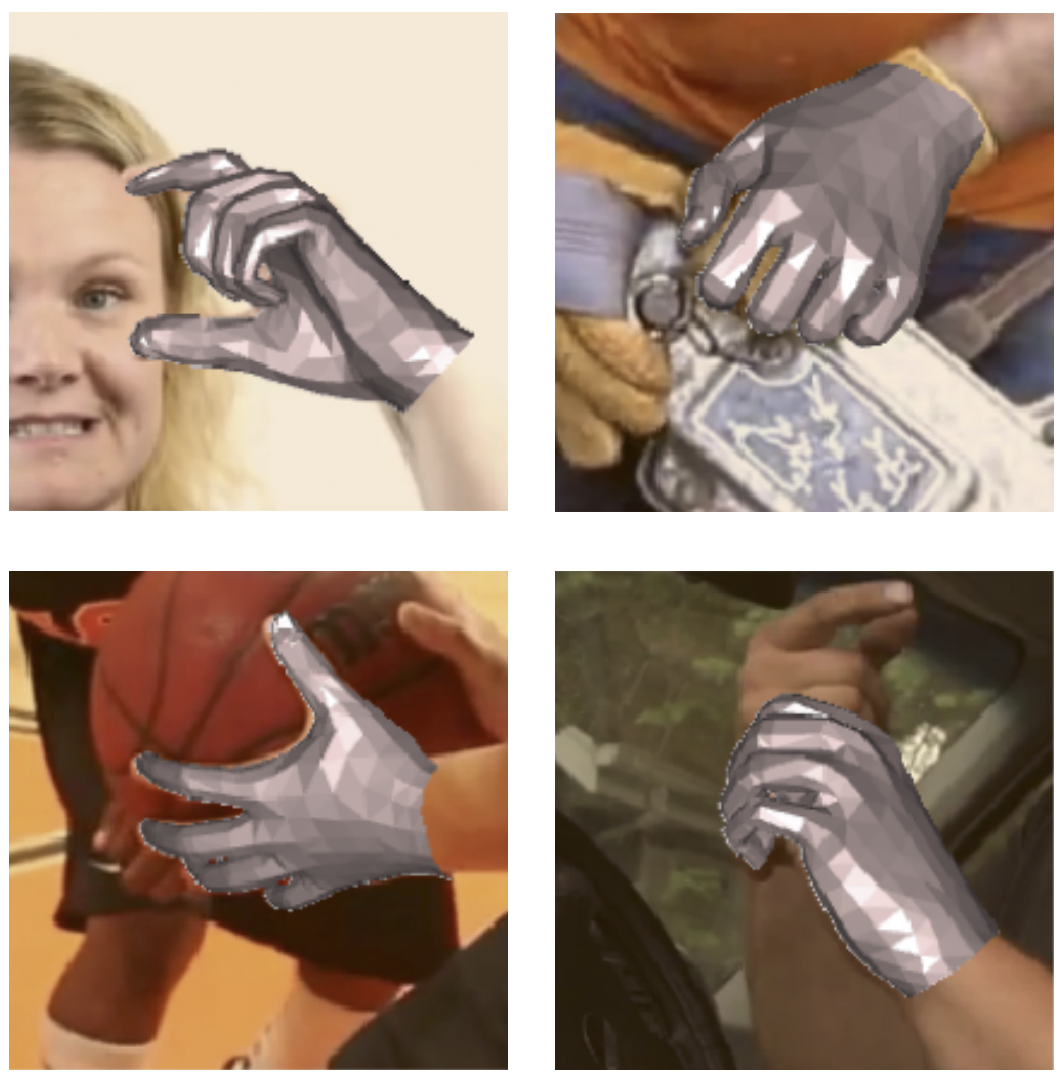
\includegraphics[width=\linewidth]{figures/ariel.png}\\ 从自然场景 2D 图像重建复杂 3D 手部姿态的示例 \citep{kulon2020weakly}。}该系统与英国初创公司 Ariel AI 合作开发，并在 CVPR 2020 上演示；它能够根据手机视频输入，以快于实时的速度创建具有完全关节化双手的逼真人体化身。%
Ariel AI 于 2020 年被 Snap 收购；在本文写作时，其技术已用于 Snap 的增强现实产品。
%Shape correspondence, Protein molecular surfaces, Ariel AI
